
\chapter{Operating parameters}
\section{Forces on a car}
	\begin{wrapfigure}[10]{l}{7.5cm}
	\vspace{-5mm}
	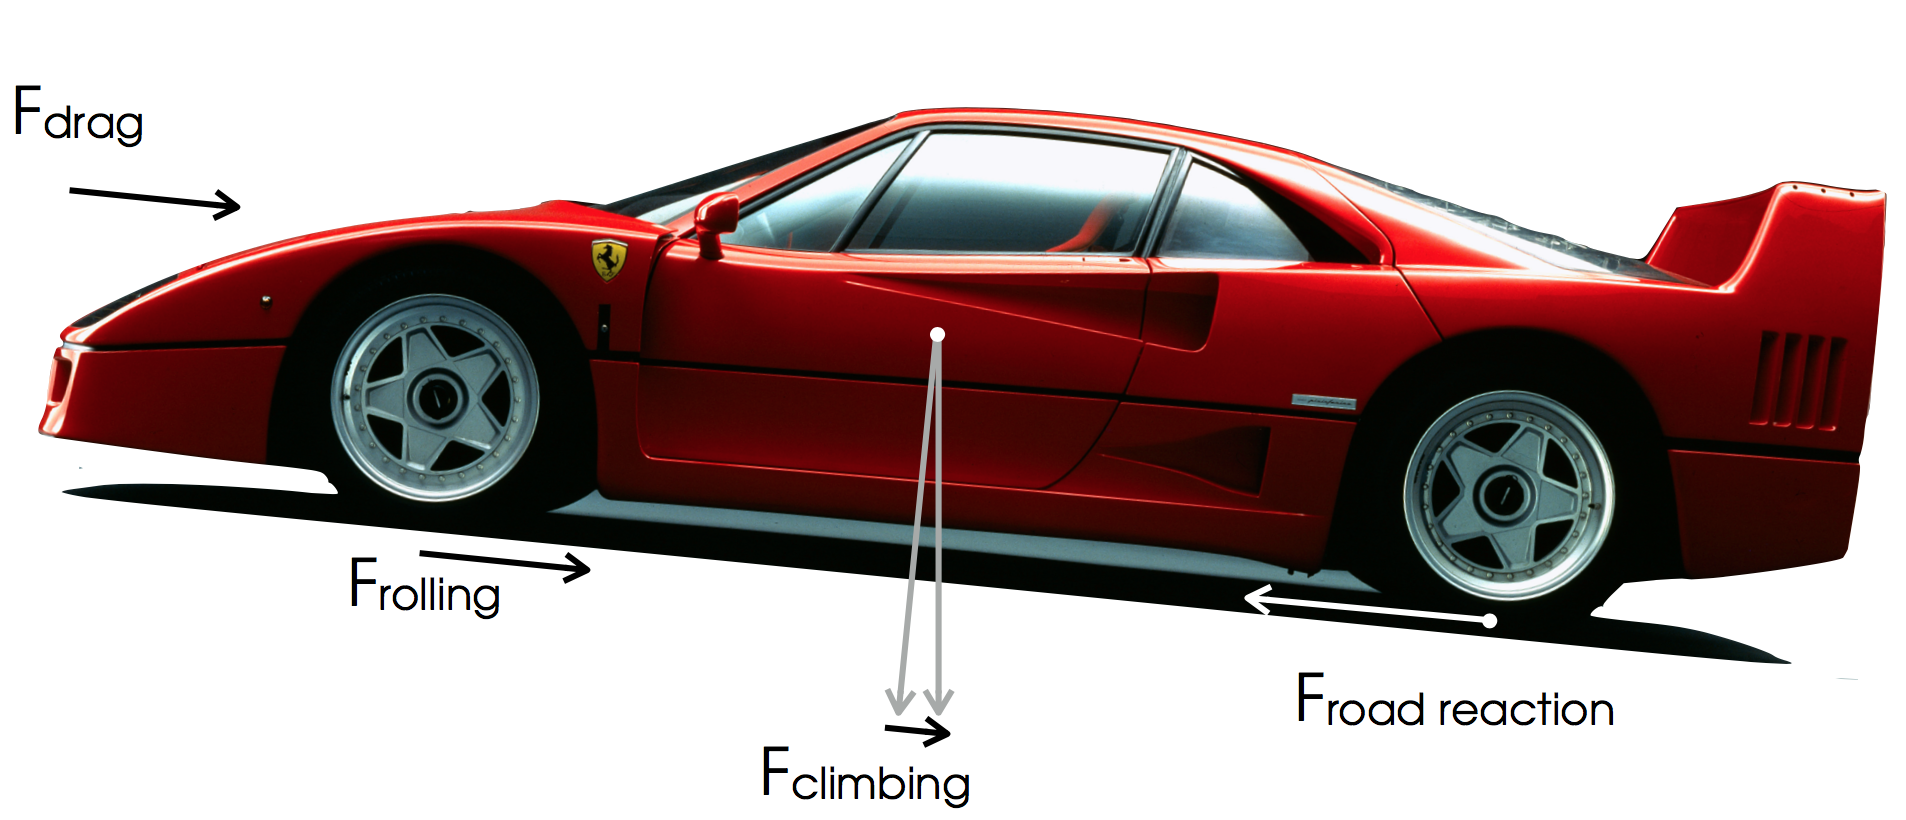
\includegraphics[scale=0.2]{ch2/1}
	\captionof{figure}{}
	\end{wrapfigure}
	The very basic, we need to apply a force to make the car move. Thus our first force is related to acceleration and energy: 
	
	\begin{equation}
	F = m.a \qquad and \qquad E= F.d
	\end{equation}
	
	This force is applied on the contact between the wheels and the road as a reaction to the torque. The three main forces opposed to the movement of the car are \textbf{rolling} of the tires, \textbf{drag} and \textbf{gravity}.
	
\subsection{The rolling force}
	\begin{wrapfigure}[6]{r}{5cm}
	\vspace{-15mm}
	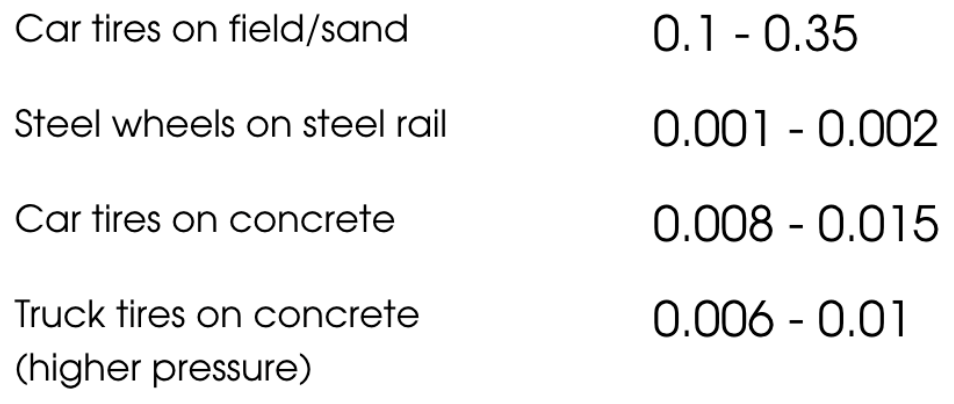
\includegraphics[scale=0.3]{ch2/2}
	\captionof{figure}{}
	\label{fig:2.2}
	\end{wrapfigure}
	The car weight of the car deforms the tire and the ground. At any time, another part of the tire and ground should be deformed and this requires a force opposed to the movement of the car. The force and the power can be characterized as:
	
	\begin{wrapfigure}[8]{l}{6.5cm}
	\vspace{-5mm}
	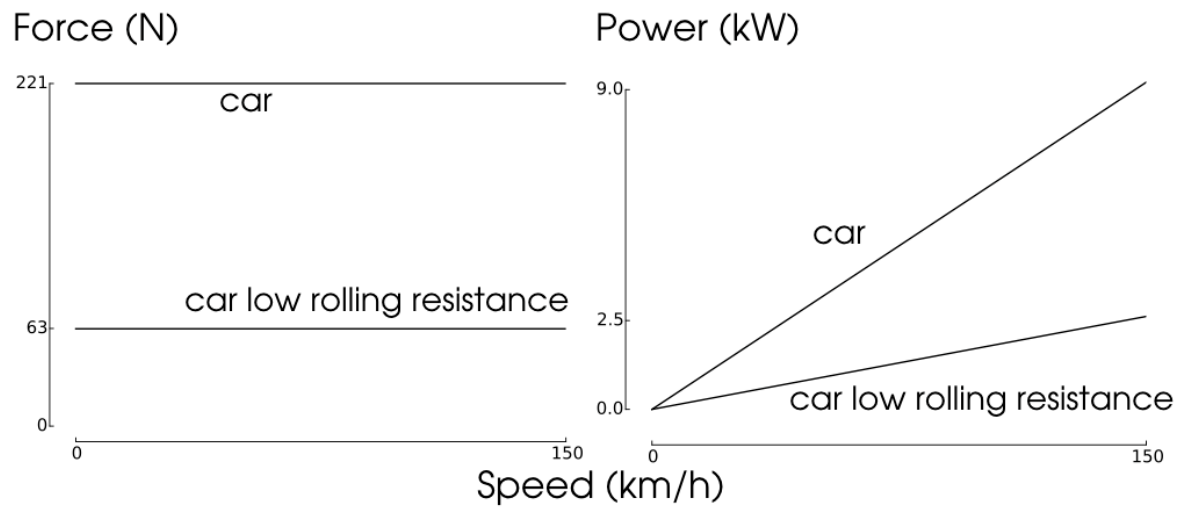
\includegraphics[scale=0.3]{ch2/3}
	\captionof{figure}{}
	\label{fig:2.3}
	\end{wrapfigure}
	\begin{equation}
	F_R = C_R m g \qquad P_R = C_R mg v
	\end{equation}
	
	where $C_R$ is the rolling resistance coefficient taking into account the effect of the deformation of ground and the tires per unit of weight applied. On \autoref{fig:2.2} we can see that the nature of both the tire and ground is important. \autoref{fig:2.3} shows the dependence of the power wrt to the velocity, while the rolling coefficient remains constant with speed. Remark that rolling power can go up to 9kW at 150 km/h. 
	
\subsection{The drag force}
	This is due to the force induced by the air opposed to the movement of the car. We have to move air particles to ride. The force and power are:
	
	\begin{equation}
	F_D = \frac{v^2}{2} \rho _a C_D A_f\qquad P_D = \frac{v^3}{2} \rho _a C_D A_f
	\end{equation}
	
	\begin{wrapfigure}[8]{l}{6.5cm}
	\vspace{-5mm}
	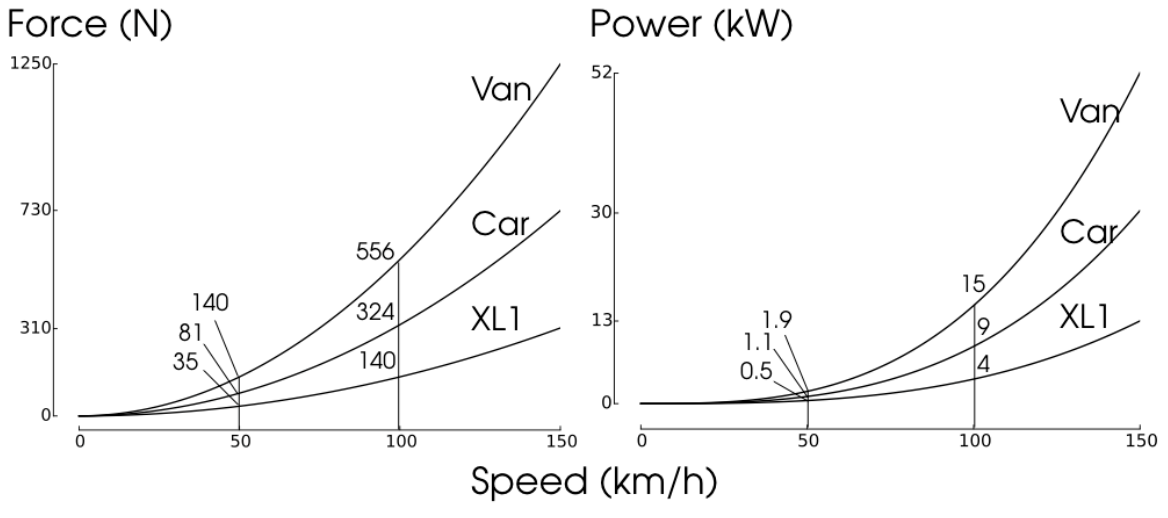
\includegraphics[scale=0.3]{ch2/4}
	\captionof{figure}{}
	\label{fig:2.4}
	\end{wrapfigure}
	where $A_f$ is the frontal area of the car and $C_D$ the drag coefficient, stating how smooth it is to move the air particles. By multiplying the drag coefficient and the frontal surface, we get another equivalent surface that gives an important factor for drag resistance. \autoref{fig:2.4} represents the evolution of the force and the power in function of the velocity, we can remark the high non-linear dependency. \\
	
	At low speed (50-60 km/h), the rolling resistance predominates. As the speed increases, the drag resistance becomes more important. Between 60-80 km/h their respective power is similar. 
	
\subsection{The climbing force}
	\begin{wrapfigure}[8]{r}{6.5cm}
	\vspace{-5mm}
	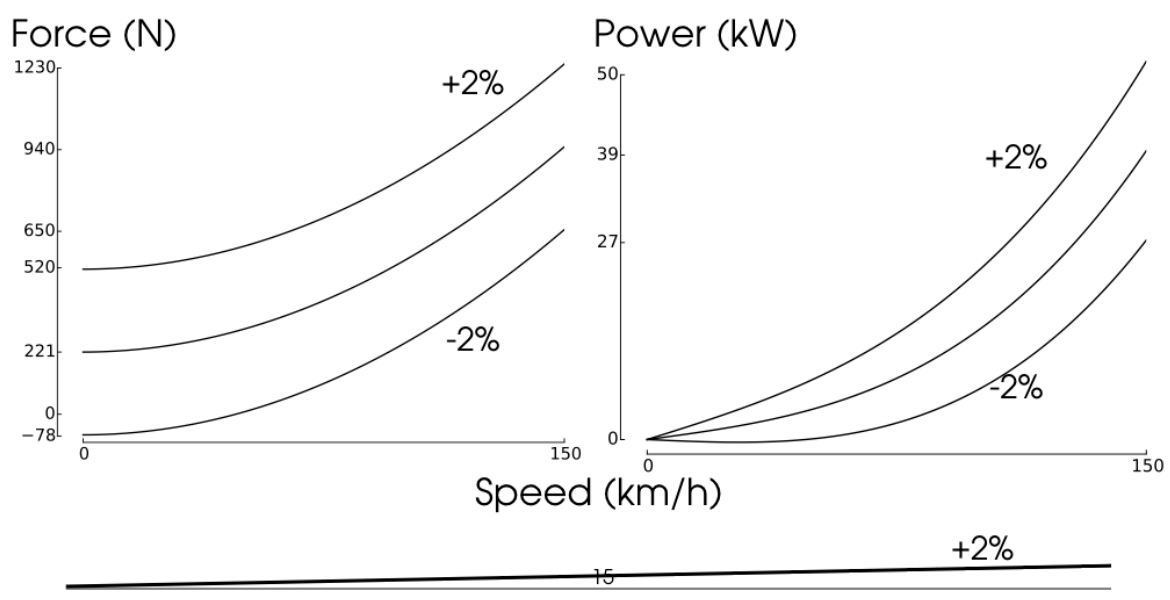
\includegraphics[scale=0.3]{ch2/5}
	\captionof{figure}{}
	\label{fig:2.5}
	\end{wrapfigure}
	This one is due to the gravity and can be expressed in function of the angle as: 

	\begin{equation}
	F_C = mg \sin \alpha \qquad P_C = mg\sin \alpha v.
	\end{equation}
	
	Let's look to \autoref{fig:2.5}, 2\% inclination can seem to be not important but the effect on the power consumption is already huge. Don't forget that energy and force are linked by the distance, going faster demands more energy. \\
	
	There are also some auxiliaries that consume energy (1-3 kW), like opening the windows or air conditioning.
	
\section{The wheels}
	\begin{wrapfigure}[11]{l}{6.5cm}
	\vspace{-5mm}
	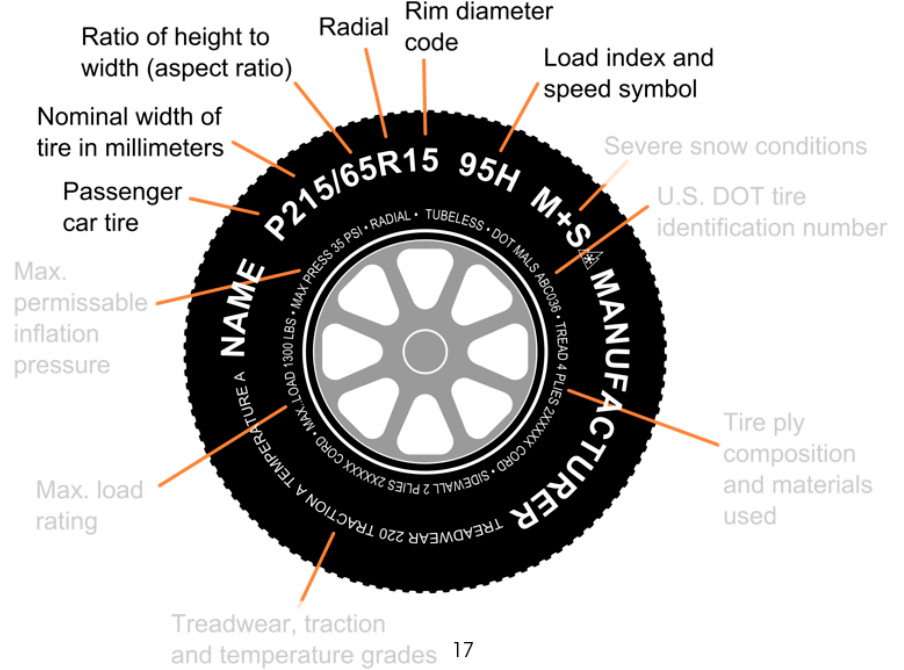
\includegraphics[scale=0.4]{ch2/6}
	\captionof{figure}{}
	\label{fig:2.6}
	\end{wrapfigure}
	To retrieve the rotational speed of the engine from the one of the car the first step is the wheels. \autoref{fig:2.6} shows the divers information on the tire. To get the real diameter in cm of the wheel we have to proceed as:
	
	\begin{equation}
	\begin{aligned}
	d (cm) &= (\mbox{rim diameter}) [inch] \cdot 2.54 [cm/inch] \\
	&+ (\mbox{width}) [mm] \cdot 0.1 [cm/mm] \cdot (\mbox{aspect ratio}) \cdot 2
	\end{aligned}
	\end{equation}
	
	Knowing this, the rotational speed of the wheel is $\omega (rad/s) = \frac{\mbox{speed (m/s)}}{d/2}$. This is the rpm of the wheel, for the one of the engine, there is the coupling with a gearbox. The power demand is lower than the supply, the \textbf{power reserve} is used for climbing and acceleration. 
	
\section{Geometrical parameters}
	\begin{wrapfigure}[4]{l}{8.3cm}
	\vspace{-5mm}
	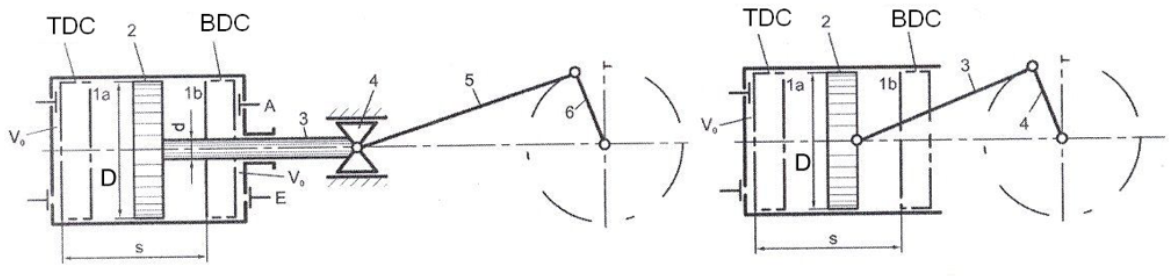
\includegraphics[scale=0.4]{ch2/7}
	\captionof{figure}{}
	\label{fig:2.7}
	\end{wrapfigure}
	We have enormous type of engine that differs from application to application by their characteristics. \autoref{fig:2.7} regroups different parts of the piston, but more important are the \textbf{dead center} at the top and the bottom which are the position of the cylinder when the velocity is null, the \textbf{bore} is the diameter of the cylinder and the \textbf{stroke} is the distance traveled by the piston. 
	
	\begin{wrapfigure}[13]{l}{7.5cm}
	\vspace{-5mm}
	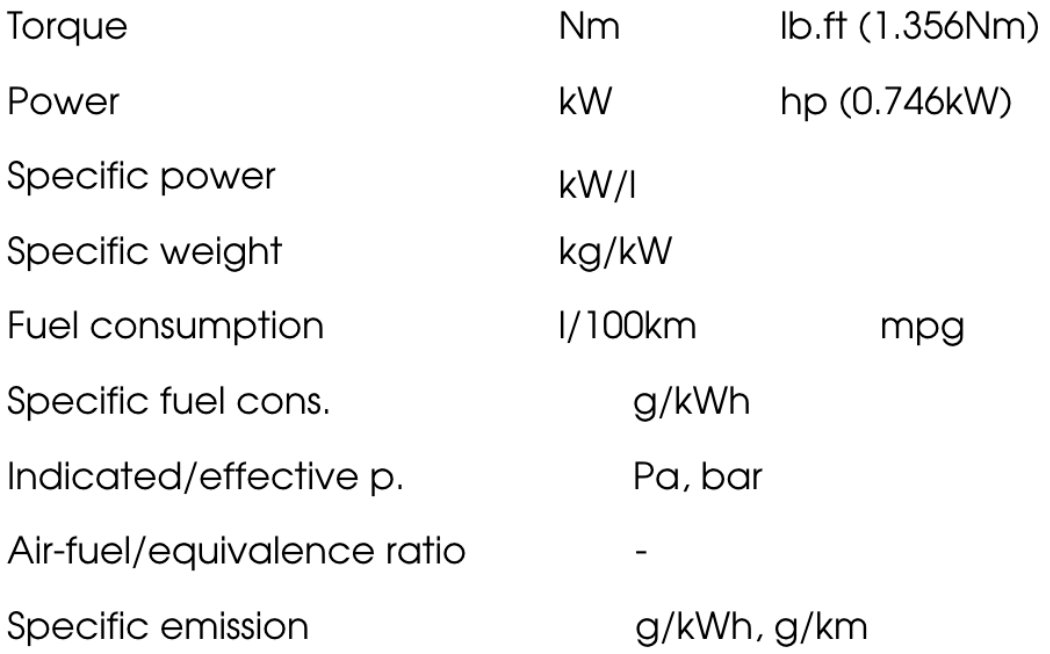
\includegraphics[scale=0.4]{ch2/8}
	\captionof{figure}{}
	\label{fig:2.8}
	\end{wrapfigure}
	We also speak about the \textbf{swept or displacement volume} and the compression ratio given by:
	
	\begin{equation}
	V_d = \pi s \frac{D^2}{4}\qquad \epsilon = \frac{V_c + V_d}{V_c}
	\end{equation}
	
	where $V_c$ is the minimum volume for valves. We have also the \textbf{mean piston speed} which is important for inertia effects, defined as:
	
	\begin{equation}
	V_m = 2s\frac{rpm}{60}
	\end{equation}

	where we remind that for one rpm we have two strokes. The rpm and $V_m$ vary a lot in function of the engine type and the application, mechanical constraints. 
	
\section{Energy conversion}
	\begin{wrapfigure}[6]{r}{5.5cm}
	\vspace{-5mm}
	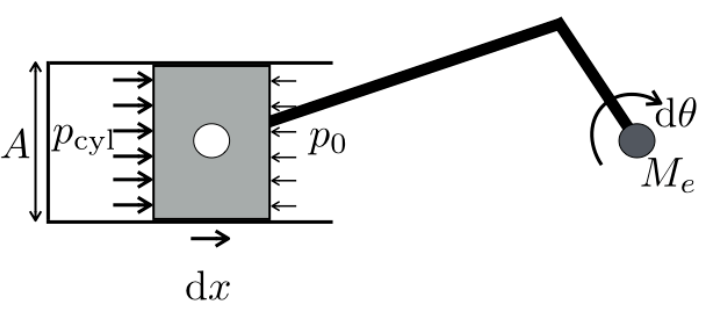
\includegraphics[scale=0.4]{ch2/9}
	\captionof{figure}{}
	\label{fig:2.9}
	\end{wrapfigure}
	As a simple model, by neglecting the inertia, friction and gravity, we can say that the energy conservation is expressed:
	
	\begin{equation}
	(p_{cyl} - p_0) A \, dx = M_e \, d\theta
	\end{equation}
	
	where the fuel energy is converted into torque. 
	
	\begin{wrapfigure}[8]{l}{4cm}
	\vspace{-5mm}
	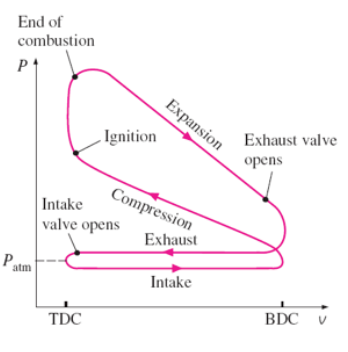
\includegraphics[scale=0.6]{ch2/10}
	\captionof{figure}{}
	\label{fig:2.10}
	\end{wrapfigure} 
	What is used to represent the engine cycle is the p-v diagram also called \textbf{Watt or indicator diagram}. We see that the exhaust phase is at higher pressure and the intake less pressure than Atm because we have to push and suck the air/fuel. The diagram of traditional engines are approximated with ideal cycles:\\ 
	
	\begin{itemize}
	\item[•] SI: Otto and Beau de Rochas cycle
	\item[•] CI: Diesel cycle
	\item[•] Dual and Sabathé cycles to better represent the diagram
	\end{itemize}
	
	
\subsection{Otto cycle}
	
	\begin{wrapfigure}[7]{r}{8cm}
	\vspace{-5mm}
	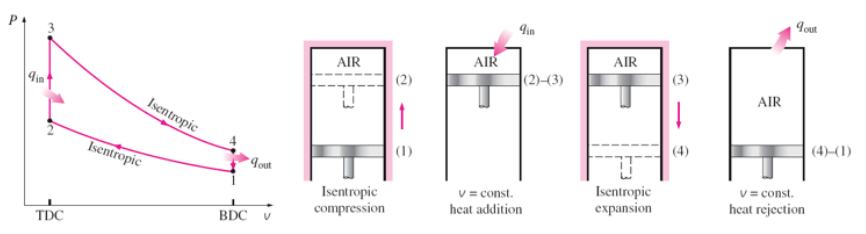
\includegraphics[scale=0.55]{ch2/11}
	\captionof{figure}{}
	\label{fig:2.11}
	\end{wrapfigure}
	In the Otto cycle, the heat is provided in a constant volume, assuming the combustion to be very fast compared to the piston speed (not realistic). The interest is the efficiency linked to the \textbf{compression ratio}:
	
	\begin{equation}
	\eta _{th} = 1 - \frac{1}{\epsilon ^{\gamma -1}}.
	\end{equation}	 
	
	\begin{wrapfigure}[5]{l}{4cm}
	\vspace{-5mm}
	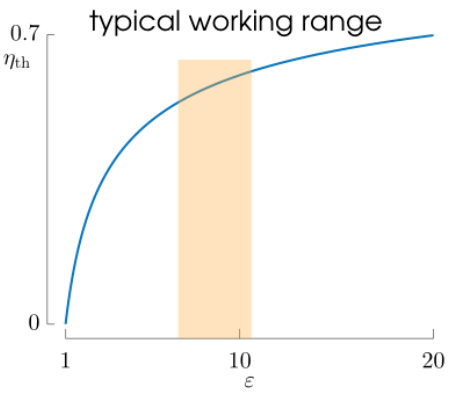
\includegraphics[scale=0.5]{ch2/12}
	\captionof{figure}{}
	\label{fig:2.12}
	\end{wrapfigure}
	We see that by increasing the compression ratio, we increase the efficiency. Unfortunately for spark ignition engines we have an upper limit due to knock. The typical working range is around $\epsilon = 10$. 	\\\\\\\\\\
	
\subsection{Diesel cycle}
	\begin{wrapfigure}[9]{r}{4cm}
	\vspace{-5mm}
	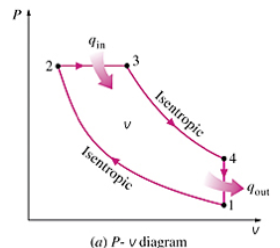
\includegraphics[scale=0.75]{ch2/13}
	\captionof{figure}{}
	\label{fig:2.13}
	\end{wrapfigure}
	In the Diesel cycle the combustion takes place when the pressure remains constant, assuming a small combustion such that the pressure increase is compensated by volume increase. In that case the $\epsilon$ is also important but there is also the \textbf{load ratio} $\alpha$:
	
	\begin{equation}
	\alpha = \frac{T_3}{T_2}= \frac{V_3}{V_2} \qquad \Rightarrow \eta _{th} = 1 - \frac{1}{\epsilon ^{\gamma -1} }\frac{\alpha ^{\gamma}-1}{\gamma (\alpha -1)} 
	\end{equation}
	
	where $T_4, T_1$ and $\alpha$ are not independent. \\
	
	\begin{wrapfigure}[8]{l}{6cm}
	\vspace{-5mm}
	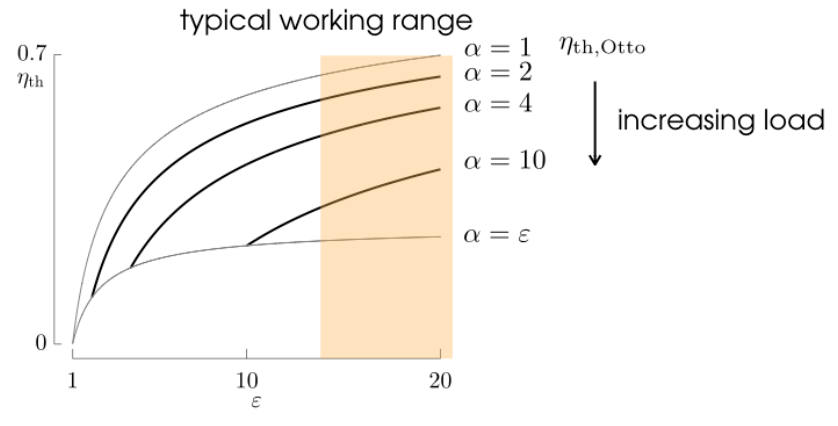
\includegraphics[scale=0.4]{ch2/14}
	\captionof{figure}{}
	\label{fig:2.14}
	\end{wrapfigure}
	We see that when $\alpha = 1$, the efficiency tends to the one of the Otto cycle. When the load increases, the efficiency decreases. For the same compression ratios, the Otto cycle is much efficient than the Diesel cycle. But we operate in much higher compression ratios in the Diesel engine because they are not limited by knock. Therefore, the efficiency of compression ignition engines is higher than the spark ignition engines: 
	
	\begin{equation}
	\eta _{th, Otto} < 	\eta _{th, Diesel}.
	\end{equation}
	
\subsection{Dual cycle}
	\begin{wrapfigure}[4]{r}{6cm}
	\vspace{-5mm}
	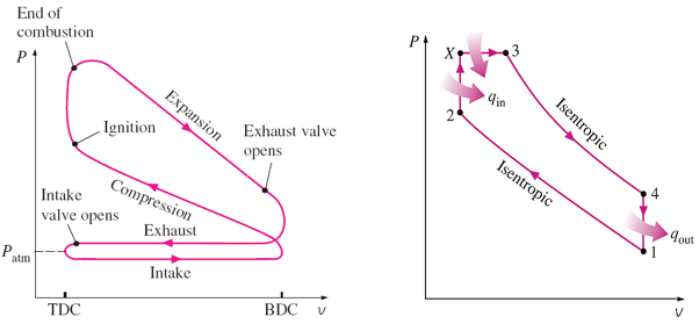
\includegraphics[scale=0.5]{ch2/15}
	\captionof{figure}{}
	\label{fig:2.15}
	\end{wrapfigure}
	The Otto cycle being too optimistic and the Diesel one too pessimistic, a good diagram should be obtained by combination of the two. However, the additional complexity does not introduce new conclusions. \\
	
\section{Power conversion steps}
	\begin{wrapfigure}[8]{l}{6cm}
	\vspace{-5mm}
	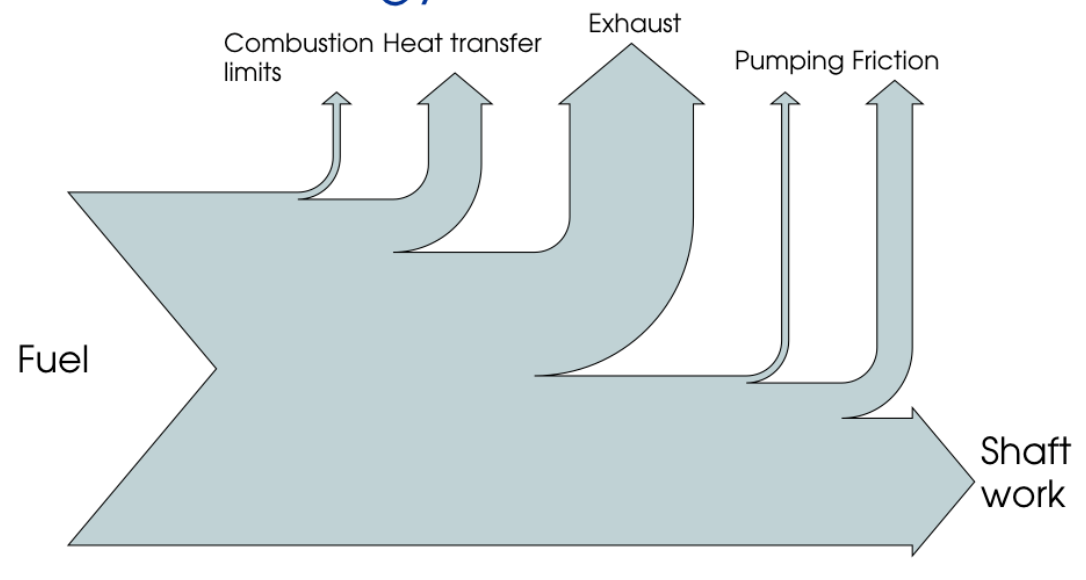
\includegraphics[scale=0.3]{ch2/16}
	\captionof{figure}{}
	\label{fig:2.16}
	\end{wrapfigure}
	Between the energy provided to the crankshaft and the power present at the fuel, there are many losses. A small part is lost in the combustion itself, a bigger part by heat transfer to the walls that are cooled down, the biggest part is lost in with the exhaust gases and we also loose when pumping and friction.  
	
\ \\\\	If we compare the indicated work $W_i$ on the p-v diagram with the energy in the fuel, we get the \textbf{indicated efficiency} (performance of the cycle):
	
	\begin{equation}
	\eta _i = \frac{W_i}{m _{fuel} LHV}.
	\end{equation}
	
	If we take into account the different losses, we get the \textbf{effective work} $W_e$. With his we can define the mechanical efficiency and the \textbf{effective efficiency} (efficiency to the crankshaft):
	
	\begin{equation}
	\eta _m = \frac{W_e}{W_i} \qquad \eta _e = \frac{W_e}{m_{fuel} LHV}.
	\end{equation}
	
	This ranges from 30\% in SI and 40\% in CI.
	
\subsection{Industry standards}
	In the industry, we represent the effective efficiency in the form \textbf{specific fuel consumption}: 
	
	\begin{equation}
	\mbox{specific fuel consumption} = \frac{\mbox{fuel mass flow }(g/h)}{\mbox{effective power} (kW)}.
	\end{equation}
	
	This last is inversely proportional to the effective efficiency. Be aware that this depends on the LHV and can change significantly when changing fuels. Note also that the $CO_2$ emission is directly linked to the fuel consumption, so the efficiency. 
	
\subsection{Pressure to work and work to pressure}
	
	
	